\documentclass{report}

\usepackage{amsmath}
\usepackage{amssymb}
\usepackage{mathtools}
\usepackage{titlepic}
\usepackage{url}
\usepackage{natbib}
\usepackage{graphicx}
\usepackage{listings}
\usepackage{color}
%\usepackage[T1]{fontenc}


\definecolor{dkgreen}{rgb}{0,0.6,0}
\definecolor{gray}{rgb}{0.5,0.5,0.5}
\definecolor{mauve}{rgb}{0.58,0,0.82}

\lstset{frame=tb,
	aboveskip=5mm,
	belowskip=5mm,
	showstringspaces=false,
	columns=flexible,
	basicstyle={\small\ttfamily},
	numbers=none,
	numberstyle=\tiny\color{gray},
	keywordstyle=\color{blue},
	commentstyle=\color{dkgreen},
	stringstyle=\color{mauve},
	breaklines=true,
	breakatwhitespace=true,
	tabsize=4
}

\lstdefinestyle{BashOutputStyle}{
	basicstyle={\small\ttfamily},
	numbers=none,
	frame=tblr,
	columns=flexible,
	breakatwhitespace=true,
	tabsize=4
}


\setlength\parindent{0pt}
\graphicspath{{./images/}}

\renewcommand{\baselinestretch}{1.5}









\begin{document}


\titlepic{
\includegraphics[scale=0.5]{DIT_logocol}}
\title{R\'{e}nyi's Parking Problem}
\author{Jerry Kiely\\
		\\
		School of Mathematical Sciences\\
		Dublin Institute of Technology\\
		Dublin 8\\
		Ireland\\
		\\
		\texttt{d16126734@mydit.ie}}
\date{\today}
\maketitle


\tableofcontents
\lstlistoflistings

\newpage





%\chapter{Summary}
%\section{Summary}
\begin{abstract}
R\'{e}nyi's parking problem is a simple random process. The expected number of cars parked, and the expected 
density of parked cars can be found in a number of ways. The author has looked at the elementary proof of 
the problem (\cite{rppr,etpp}), and provided a simulation to evaluate R\'{e}nyi Parking Constant. \bigskip
\end{abstract}





\chapter{Background}
%\section{Background}

The problem statement is as follows: consider an interval $(0, x)$ upon which we place a segment of unit 
length at random. We continue by placing a second segment of unit length randomly upon the original 
interval, discarding the segment if it overlaps with the original one. \bigskip

We continue in this fashion until we can no longer add unit segments without overlap. At each step the 
next position within the interval is chosen from a uniform distribution of the remaining locations within 
the interval. \bigskip

We are interested in both the expected value of the number of unit segments contained within the interval 
$(0, x)$, denoted $M(x)$, and the expected filling density of unit segments within the interval, denoted 
$M(x) / x$. \bigskip






\chapter{Methods}
%\section{Methods}

Before proceeding with the simulations, let us look at the derivation of the equation for $M(x)$. If we 
initially consider an interval $(0, x + 1)$ and upon this place a unit segment $(t, t + 1)$. This unit 
segment partitions the original interval into two smaller intervals - $(0, t)$ and $(t + 1, x + 1)$. So 
the expected number of unit segments contained within the original interval is: \bigskip

\[
	M(x + 1) = M(t) + 1 + M(x - t)
\]\medskip

where $1$ represents the expectation of added segment within the unit interval $(t, t + 1)$. Integrating 
with respect to $t$ we get: \bigskip

\begin{eqnarray*} 
	\int_{0}^{x} M(x + 1) dt & = & \int_{0}^{x} [M(t) + 1 + M(x - t)] dt \\
    M(x + 1) \int_{0}^{x} dt & = & \int_{0}^{x} dt + \int_{0}^{x} [M(t) + M(x - t)] dt \\
            M(x + 1) \cdot x & = & x + \int_{0}^{x} [M(t) + M(x - t)] dt \\
	                M(x + 1) & = & 1 + \frac{1}{x} \int_{0}^{x} [M(t) + M(x - t)] dt 
\end{eqnarray*}\medskip

as the distributions within each of the smaller intervals are uniform, and hence the same, we get: \bigskip

\[
	M(x + 1) = 1 + \frac{2}{x} \int_{0}^{x} M(t) dt
\]\medskip

changing variables we get: \bigskip

\[
	M(x) = 1 + \frac{2}{x - 1} \int_{0}^{x - 1} M(t) dt
\]\medskip

more completely, and because adding a unit segment to an interval of length less than $1$ has no meaning, 
the equation for $M(x)$ can be written as: \bigskip

\[
	M(x) = 
	\begin{dcases}
		0,                                            & \text{for } 0 \leq x < 1 \\
		1 + \frac{2}{x - 1} \int_{0}^{x - 1} M(t) dt, & \text{for } x \geq 1
	\end{dcases}
\]\medskip






\chapter{Results}
%\section{Results}

Both the elementary proof and the recurrence form above allows one to write a simulation. We write a function 
that does the following: \bigskip

\begin{itemize}
	\item find a parking spot  in the interval using a uniform distribution
	\item the found parking spot partitions the interval into two
	\item recursively calls itself on the two partitions
	\item returns if the partition size is less than $1$
\end{itemize}\medskip

\begin{lstlisting}[language=Python, caption=Parking problem function]
def parking_problem(length):
	spots = []
	
	def find_spots(start, end):
		spot = np.random.uniform(start, end - 1.0)
		spots.append(spot)
		
		if spot - start >= 1.0:
			find_spots(start, spot)
		
		if end - spot >= 2.0:
			find_spots(spot + 1.0, end)
	
	find_spots(0, length)
	
	return len(spots) / float(length)
\end{lstlisting}\medskip

This function exits when no more candidate spots remain. A second function aggregates the results of the 
simulation function in order to calculate statistics. \bigskip

\begin{lstlisting}[language=Python, caption=Simulation function]
def simulation(iterations, length):
	results = []
	
	for i in range(iterations):
		results.append(parking_problem(length))
	
	return results
\end{lstlisting}\medskip

The simulation produces the following output: \bigskip

\begin{lstlisting}[style=BashOutputStyle, caption=Simulation output]

[ jerry@ponocrates ~ ] $ python3 parking_problem.py 1000 1000000

     Parking Problem: running 1000 simulations...
                      : iteration  1000
                      : simulations completed...

     Parking Problem: results
        Distribution:
                 mean: 0.7476
  standard deviation: 0.0001

\end{lstlisting}\medskip

and a plot of the results can be seen below. As can be seen the estimate for the R\'{e}nyi number is around $0.7476$: \bigskip

\begin{figure}[h]
	\centering
	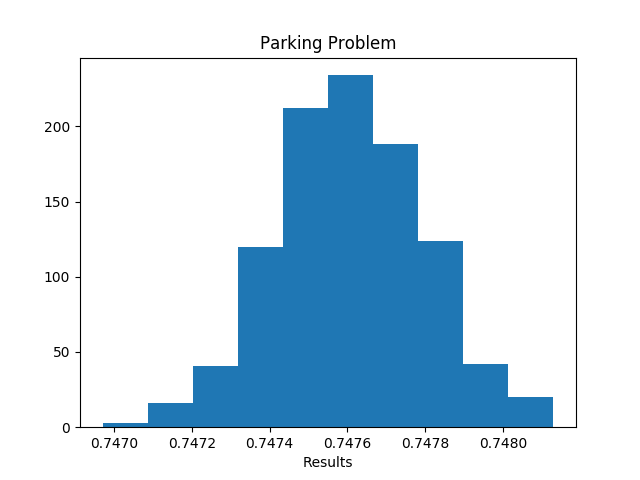
\includegraphics[scale = 0.75]{parking_problem_1000}
	\caption{The Parking Problem Result Distribution}
	\label{fig:tppd}
\end{figure}\medskip




\chapter{Comments}
%\section{Comments}

There are many approaches to solving the parking problem, and there are also many variations of this problem: \bigskip

\begin{itemize}
	\item the discrete parking problem
	\item the two dimensional random sequential packing problem
	\item the three dimensional random sequential packing problem
	\item the parking problem with segments of different length
	\item the reversible parking problem 
\end{itemize}\medskip

One of the more interesting applications is the theory of Random Sequential Adsorption (RSA). This can describe the 
adsorption of particles onto a substrate. These particles include proteins, bacteria, gas molecules, polymers, colloids, 
and more. \bigskip




\newpage

\bibliographystyle{plain}
\bibliography{bibtex/bibliography}

\end{document}
